% !TEX root = ../thesis_main.tex
\chapter{Coherent Processes of Single-Wall Carbon Nanotubes}

\section{Introduction}


{\color{red} UNFINISHED}Talking about ultrafast optical switching. SWCNTs quite suited to this due to fast carrier dynamics, unlike those of inorganic semicondutors \cite{maeda2006gigantic}. Useful for optical switching processes such as those induced by the optical Stark effect. However, multi-photon processes occur that lead to the creation of real carriers which can photo-bleach the $E_{11}$ resonance if enough carriers are created and thereby limit the performance of the optical switching.

We can quantify the performance of optical switching by using the term reversibility to describe the effect on which non-coherent processes on the optical switching. Here, reversibility is defined as
%
\begin{equation}
 	\text{Rev} = \dfrac{\Delta T_\text{peak} - \Delta T_\text{base}}{\Delta T_\text{peak}},
\end{equation}
%
which includes the baseline transmission $\Delta T_\text{base}$ that represents the average of the transmission before and after switching occurs whereas, the peak change in transmission $\Delta T_\text{peak}$ only measures the coherent changes in transmission due to the optical Stark effect. Furthermore, $\Delta T_\text{base}$ accounts for changes in trasmission due to the creation of real carriers. It also implicitly depends on other parameters such as the detuning and fluence of the optical pump as well as the time delay between incident pump pulses.

{\color{red} UNFINISHED} Theory developed by Professor Mackillo Kira and his student Weiwei Jiang. Here, they solve Maxwell-semiconductor Bloch equations \cite{kira2011semiconductor, hirtschulz2008carbon} in a self-consistent manner for (6,5) SWCNTs. The semiconductor Bloch equations include
%
\begin{equation}
	\begin{split}
	i \hbar \frac{\partial}{\partial t} P_\text{k} &= \tilde{E}_\text{k} P_\text{k} - ( 1- f^\text{e}_\text{k} - f^\text{h}_\text{k})\Omega_\text{k} + \Gamma_\text{k}, \\
	\hbar \frac{\partial }{\partial t} f_\text{k}^\text{e(h)} &= 2 \text{Im}[P_\text{k}\Omega_\text{k}^*] + \Gamma^\text{e(h)}_\text{k}
	\end{split}
\end{equation}
%
 In a typical scenario, the optical pump pulse creates an electron (hole) distribution $f_\text{k}^\text{e(h)}$, via multi-photon processes, as well as a coherent polarization $P_\text{k}$ at the carrier momentum $\hbar k$. The term $\Gamma_\text{k}$ accounts for the Coulomb interactions between the carrier distributions and the initial coherent polarization. Moreover, the variable $\tilde{E}_\text{k}$ defined as
%
\begin{equation}
	\tilde{E}_\text{k} = E_\text{k} - \sum_\text{k'} V_\text{k - k'} ( f_\text{k'}^\text{e} + f_\text{k'}^\text{h}),
\end{equation}
%
refers to the renormalized electron-hole energy. This includes the bangap energy $E_\text{k}$ as well as the Coulomb matrix element $V_\text{k}$. In addition, $\Omega_\text{k}$ refers to the renormalized Rabi energy given as
\begin{equation}
	\Omega_\text{k} = d_\text{k} \cos\theta E(t) + \sum_\text{k'} V_\text{k - k'} P_\text{k'},
\end{equation}
whichi includes the matrix dipole element $d_\text{k}$, the electric field of the optical pump $E$ and the angle $\theta$ between the polarization of $E$ and the dipole moment associated with $d_\text{k}$. In the computations, these semiconductor-Bloch equations are coupled directly to Maxwell's equations.

These calculations also account for non-coherent processes to help describe the dephasing kinetics which may affect the reversibility of the optical switching dynamics. Shortly after the initial photo-excitation, $P_\text{k}$ begins to dephase due to scattering events within the $f_\text{k}^\text{e(h)}$ distribution as a result of Coulomb interactions. From a phenomenological perspective, this dephasing can be described by an instantenous decay
\begin{equation}
	\dfrac{\partial}{\partial t} P_\text{k}(t) \Big|_\text{instant} = -\gamma P_\text{k}(t),
\end{equation}
which is parametrized by a dephasing constant $\gamma$ that implicitly accounts for quantum-kinetic scattering. However, after taking a full account of the quantum phenomena underlying these behaviors
%
\begin{equation}\label{eq:kira_phenom_dephase}
	\dfrac{\partial}{\partial t} P_\text{k}(t) \Big|_\text{Q. Memory} = -\gamma \int^{t}_{\infty} dt' \left[ \exp\left\{ - \frac{\small i}{ \small \hbar} \hat{\mathcal{H}}_\text{ex}(t-t') \right\} P(t') \right]_\text{k} \exp \left(- \frac{t-t'}{T_\text{QM}} \right).
\end{equation}
%
In this expression, the exponential term parametrized by the Hamiltonian $\hat{\mathcal{H}}_\text{ex}(t-t')$ propagates the excitonic polarization forward in time. This Hamiltonian is expressed as
\begin{equation}\label{eq:kira_quantum_dephase}
	\left[ \hat{\mathcal{H}}_\text{ex} \right]_\text{k, K}= \delta_\text{k, K} \tilde{E_\text{k}} - (1 - f_\text{k}^\text{e} - f_\text{k}^\text{h}) V_\text{k-K},
\end{equation}
%
and acts as an effective Hamiltonian for excitons in the system. The other more curious term $T_\text{QM}$ defines the duration of the quantum memory.

Quantum memory, using light as a carrier of information and encoding this information into matter \cite{iakoupov2013efficient}. Quantum memory here refers to the system's memory of the irradiation caused by optical pump, stored within $P_\text{k}$, that can be retrieved by measuring the transmission of the optical probe. Experiments suggest that $T_\text{QM} = $ 66 fs. Ultrafast switching applications, prefer to have shorter duration to facilitate optical switching on a picosecond timescale or faster.
\section{Experimental Results}

\begin{figure}[H]
	\centering
	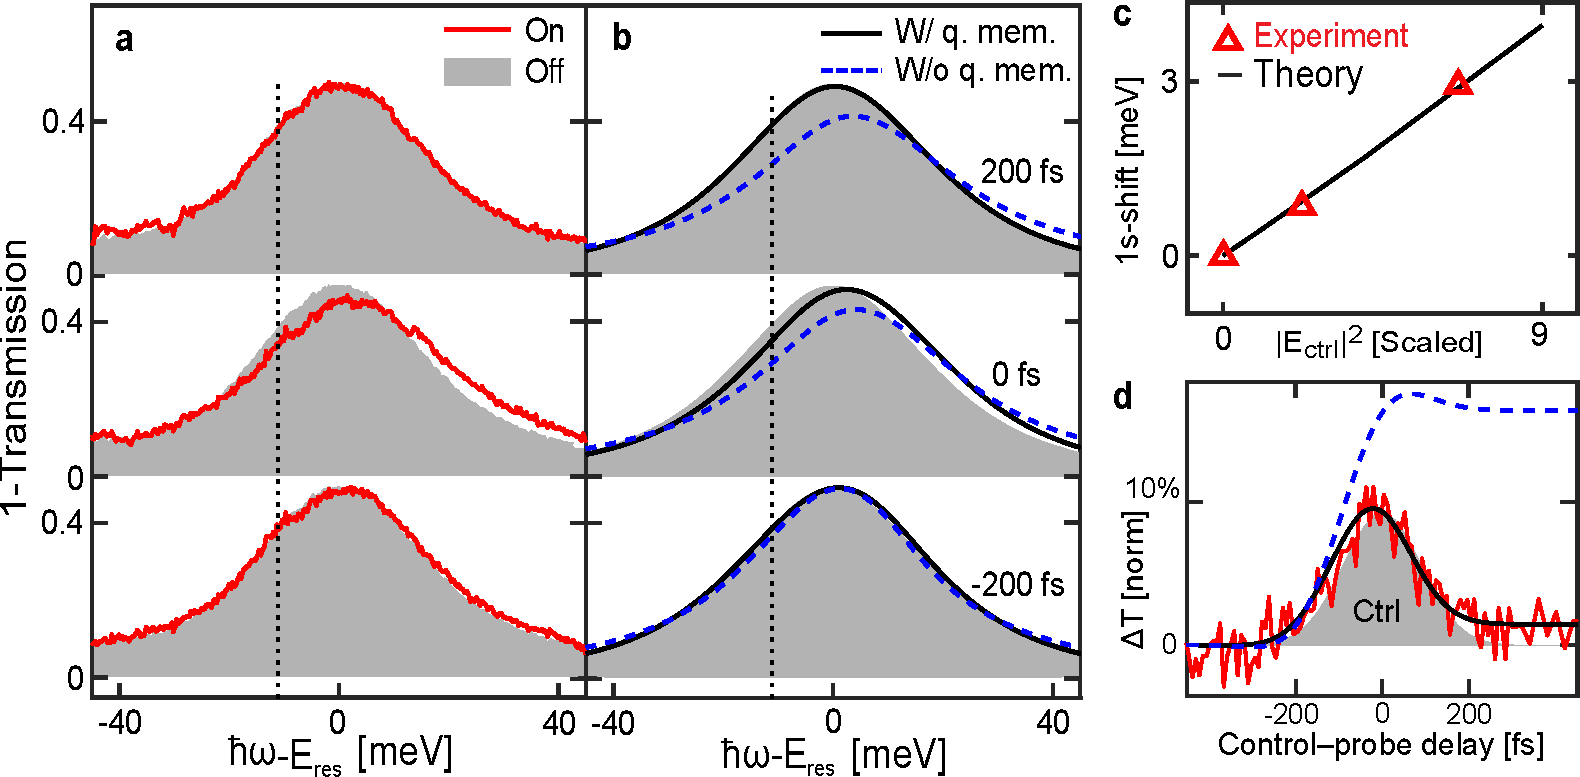
\includegraphics[height=2.6in]{images/chapter_coherent/nonresonant}
	\caption{(a) Measured vs.\ (b) numerically simulated transmission spectra of the SWCNT ensemble both with (solid lines) and without (shaded area) the influence of the optical pump beam. The dashed line shows how the transmission spectrum would evolve by using the phenomenological description of the dephasing dynamics represented in Equation \eqref{eq:kira_phenom_dephase} as opposed to the quantum-kinetic approach given by Equation \eqref{eq:kira_quantum_dephase}. Without considering quantum memory, the $E_{11}$ resonance becomes slightly photo-bleached and shifts in a non-coherent fashion. However, the quantum-kinetic description that includes quantum memory agrees with the experimental data. (c) Calculated (solid line) vs. experimentally measured Stark shift $\Delta E$. The Stark shift scales linearly with the intensity of the optical pump beam expressed as $|E_\text{ctrl}|^2$ (d) Time-resolved differential transmission probed at the $E_{11}$resonance. The shaded area represent the temporal profile of the optical pump pulse. The curves correspond to experimental data (solid red line), a theoretical calculation including quantum memory (solid black line) and another computation excluding the effects of quantum memory (dashed blue line). Reproduced from Ref.\ \cite{mack2019}}
\end{figure}

\begin{figure}[ht]
	\centering
	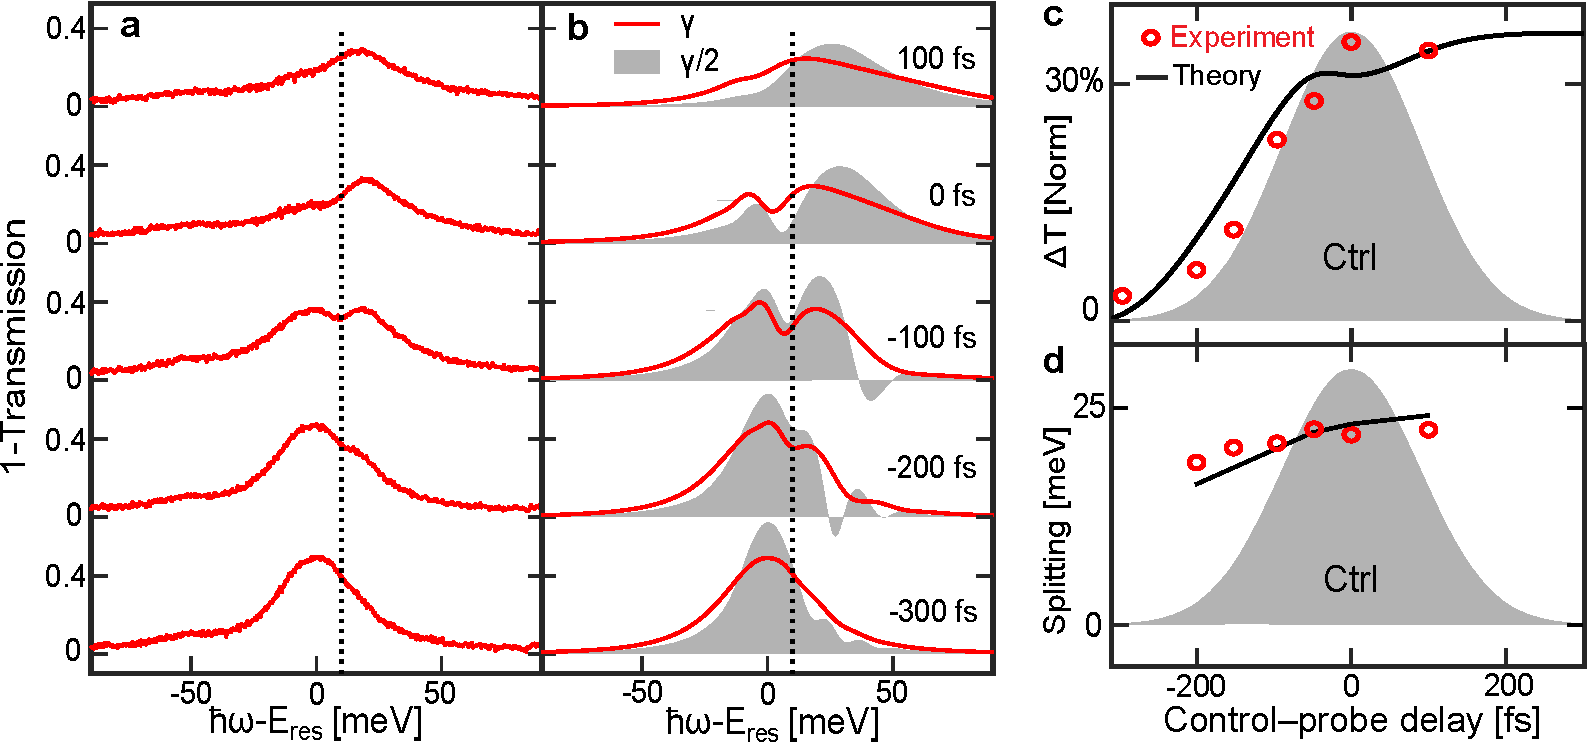
\includegraphics[height=2.6in]{images/chapter_coherent/resonant}
	\caption{{\color{red}UNFINISHED} Simulation of ultrafast switching reversibility. (a) Calculated differential transmission within the span of eight 200fs optical pulses irradiating the system. The shaded  Reproduced from Ref.\ \cite{mack2019}}
\end{figure}

\clearpage

\begin{figure}[ht]
	\centering
	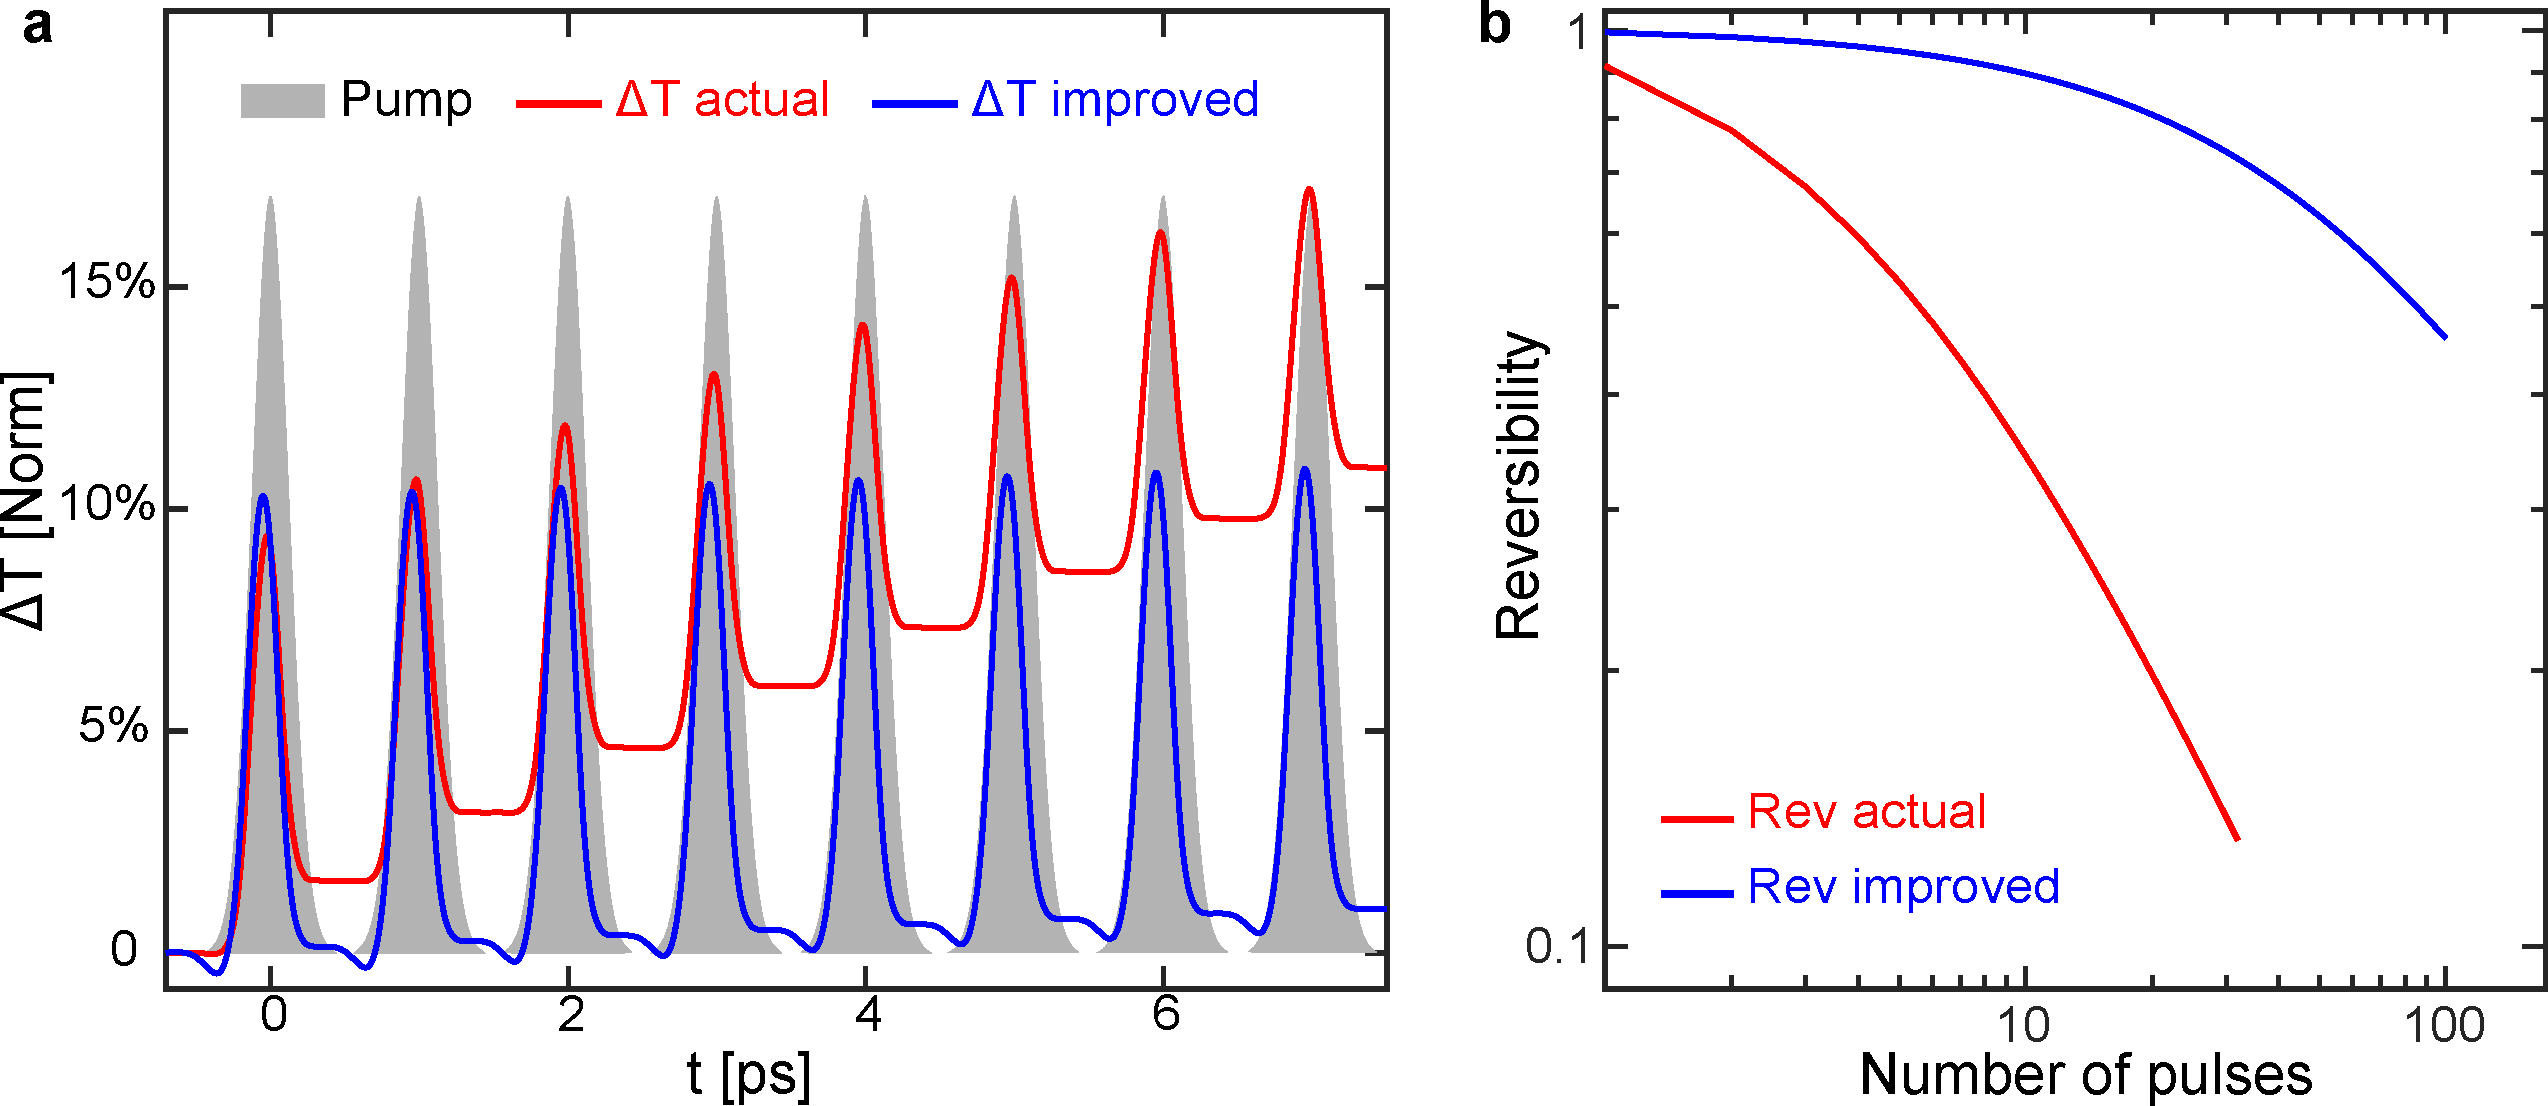
\includegraphics[height=2.6in]{images/chapter_coherent/switching_reversibility}
	\caption{{\color{red}UNFINISHED} (a)  Reproduced from Ref.\ \cite{mack2019}}
\end{figure}




\section{Discussion}

\section{Conclusions}
